\documentclass[Main]{subfiles}
\begin{document}

\section{Generelle designbeslutninger}
Undervejs i projektet skulle der tages nogle beslutninger for, hvordan arkitekturen på nye elementer skulle opstilles og hvordan filerne skulle skrives. 
Det følgende afsnit beskriver de største beslutninger og alternativer der blev overvejet.

\subsection{Én eller flere mapper}\label{Sec:en-flere}
Den rå kode hentet fra AeroQuad's Github repository \cite{Github-AQ} er opbygget med de største og mest essentielle filer i én mappe, mens alle hardware-specifikke filer er gemt i en anden mappe, med hver sin undermappe.
Dette skyldes Arduino's IDE, Sketch, kun læser filer fra én bestemt placering der ikke er det samme som projektets \code{.ino}-fil (kan sammenlignes med Visual Studio's \code{.sln} på nogle punkter).

Projektet gemmes i gruppens eget Github repository \cite{Github-IHA} og kræver derfor filerne ligger under den samme hovedmappe.
Da dette strider imod Arduino's obligatoriske opbygning, skulle hver fil kopires til den korrekte mappe, ændres og kopires tilbage.
For at undgå dette blev det forsøgt at lave et symlink\cite{symlink} mellem den obligatoriske mappe, \code{/Arduino/libraries}, og gruppens egen mappe, \code{Drone/Kode/AeroQuad-master/Libraries}, således Arduino-mappen kiggede i gruppens mappe fra sit eget link.

Dette virker desværre heller ikke, da det at have to mapper er en kunst i sig selv.
Løsningen på problemet blev derfor at flytte samtlige filer til samme mappe som \code{.ino}-filen.



\subsection{Med eller uden .cpp-filer}\label{Sec:cpp-filer}
Som beskrevet i afsnit \ref{Sec:en-flere} lå de hardware-specifikke filer i hver sin undermappe og bestod udelukkende af \code{.h}-filer, hvilket vil sige at definition og implementering lå i samme fil.
Dette er imod all gode kodestandarder, men det vil være en tidskrævende process at omskrive dem alle og teste, at de stadig virkede efter hensigten.
Derfor blev der videreudviklet i samme stil den første uge, indtil adskillige tusind fejl begyndte at vælte frem.

Problemets kerne lå i, at \code{.h}-filer med Arduino-konfiguration afvikles med en \code{C}-kompiler og ikke en \code{C++}-kompiler, hvilket var nødvendigt for nogle af de tilføjede og essentielle filer i systemet.

Løsningen bestod derfor i, at opdele samtlige filer i \code{.h}-filer og \code{.cpp}-filer, da slutningen på filnavnet er nok til, at aktivere \code{C++}-kompileren.



\subsection{Hierakisk opbygning}

\begin{wrapfigure}{r}{0.25\textwidth}
  \vspace{-20pt}
  \begin{center}
	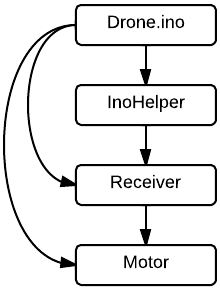
\includegraphics[scale=0.6]{Hierarki}
  \end{center}
  \vspace{-20pt}
  \caption{AeroQuad's opbygning.}
  \label{Fig:Hierarki}
  \vspace{-20pt}
\end{wrapfigure}

Under omskrivning af koden i afsnit \ref{Sec:cpp-filer} stod det klart, at Aero\-Quad's kode versus normal \code{C++}-kode ikke bruger den samme form for \code{\#include}.
Hvor normal \code{C++}-kodeskik siger, at en klasse ikke behøver vide mere end lige præcis det den skal, har AeroQuad valgt at lade \code{.ino}-filen kende til samtlige filer, vist på Figur \ref{Fig:Hierarki}.

Dette bliver et problem, når der skal holdes styr på kald til forskellige klasser, og det øverste fillag tager fat i det nederste, for dette kan overskrive alle funktioners arbejde.

Det er en stor process at omskrive samtlige filer til, kun at indeholde hvad de skal og intet ekstra og dette blev derfor fortaget løbende som fejlene blev fundet.
Dette blev især vigtigt, da klassen for beslutninger om, hvad dronen skulle foretage sig ved forskellige radio-kommandoer skulle skrives.


\subsection{Beslutningstager i C}
\begin{wrapfigure}{r}{0.30\textwidth}
  \begin{center}
	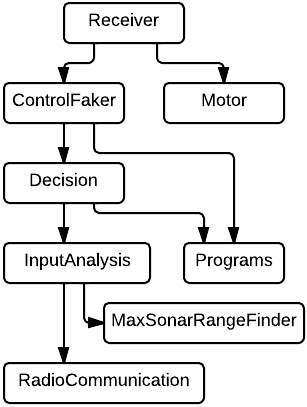
\includegraphics[scale=0.6]{Decision}
  \end{center}
  \vspace{-20pt}
  \caption{Beslutningstagning.}
  \label{Fig:Decision}
  \vspace{-10pt}
\end{wrapfigure}

Dronen er købt til, at holde sig selv i luften og tage flyve ud fra signaler fra en fjernbetjening til droner.
Det betyder, at påmontering af et ekstra sæt sonarsensorer og en radio, som dronen skal tage valg fra, skal simuleres som var det fjernbetjeningen der sendte kommandoerne.

For at beholde forståelsen for systemet blev det bygget som en spike, således, at der først blev taget hånd om, at modtage data fra radioen.
Herefter blev der sat nogle grænser for, hvad dataen måtte være mere eller mindre end for sonar og disse kunne rejse nogle flag, samt validering af radiokanalen.
Til sidste skulle der træffes en beslutning for, hvilket program der skulle afvikles og sendes return som input for fjernbetjeningen.

Selve beslutningen kan laves på flere metoder og den mest oplagte vil at bruge et \code{map}, således alle input, og kombinationer heraf, vil lede til nogle få kommandoer der skulle udføres.
\code{Map}\dots




































\end{document}